% ---------------------------------------------------------------- 23 Nov 2026: why the GA (Z2 = ga7c3, Z3 = ga8c8) keeps SBT ring 2 and drops 0, 1, 4
\begin{btframe}{7 · Back-up · Z2 SBT rings}{Z2 design: which SBT rings the optimiser keeps, and why}
\noindent \begin{minipage}[t]{\dimexpr(0.47\linewidth-0.47\dimexpr9.67pt\relax)}\vspace{0pt}\centering
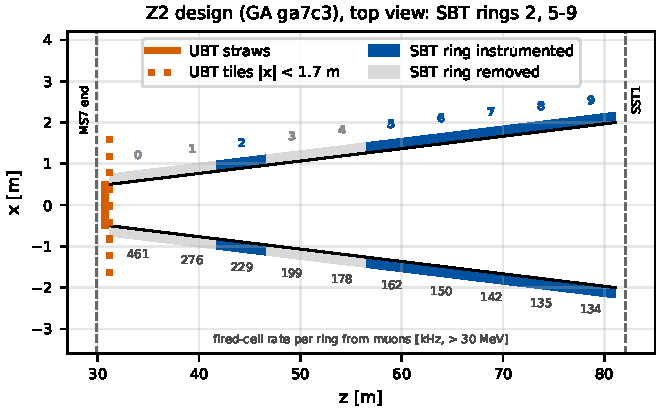
\includegraphics[width=\linewidth,height=150pt,keepaspectratio]{figs/s46_z2_design_top.pdf}\par
\end{minipage}%
\hfill%
\begin{minipage}[t]{\dimexpr(0.53\linewidth-0.53\dimexpr9.67pt\relax)}\vspace{0pt}\raggedright
\begin{itemize}
  \item \textbf{Z2} (GA ga7c3): SBT rings 2, 5–9; \textbf{Z3} (ga8c8): 2, 3, 5–9. Both drop 0, 1, 4
  \item From the 104 GA designs of run ga\_20261119\_115533; backgrounds per 15 y after the veto
\end{itemize}
\vspace{2pt}
{\fontsize{5.02pt}{6.52pt}\selectfont\setlength{\tabcolsep}{3.2pt}\renewcommand{\arraystretch}{1.42}
\begin{tabularx}{\linewidth}{lrr>{\raggedright\arraybackslash}X}
\textcolor{muted}{ring} & \textcolor{muted}{z [m]} & \textcolor{muted}{cells [kHz]} & \textcolor{muted}{effect of the ring in the GA} \\\headrule
0 & 31.1–36.9 & 461 & on: SBT-material bkg 2.9 ± 2.9 (\textbf{1 MC event} in its LS), off: 0.004 \\\rowrule
1 & 36.9–41.8 & 276 & no background gained; +27 drachmas, +0.3 \% signal lost \\\rowrule
\rowcolor{tint}\bfseries 2 & \bfseries 41.8–46.7 & \bfseries 229 & \bfseries MS7 μ V0 needs one of rings 1–3: rings 0–4 off 1.4×10\textsuperscript{4}, ring 2 on 0.80 \\\rowrule
3 & 46.7–51.6 & 199 & marginal next to ring 2 (Z3 keeps it) \\\rowrule
4 & 51.6–56.5 & 178 & sees 7 \% of the MS7 events missed by 5–9 \\\rowrule
5–9 & 56.5–81.1 & 162–134 & kept by every good design \\\rowrule
\end{tabularx}\par}
\vspace{2pt}
\begin{itemize}
  \item Ring 0 is removed for one heavy MC event: the SBT material exists only where there are cells
  \item Running: ×11 LS statistics (10 new samples) to test that event
\end{itemize}
\end{minipage}\par
\end{btframe}
